\documentclass[12pt,a4paper]{scrreprt}

\usepackage{cmap}
\usepackage[T1]{fontenc} 
\usepackage[utf8]{inputenc}
\usepackage[english,russian]{babel}

\usepackage{caption}
\usepackage{subcaption}
\usepackage[normalem]{ulem}

%\usepackage{soulutf8}

\usepackage{float}

\usepackage{enumitem}

\usepackage{graphicx}
\usepackage{multirow}


\usepackage{pgfplots}
\pgfplotsset{compat=newest}
\usepgfplotslibrary{units}


\usepackage{caption}
\captionsetup{labelsep=endash}
\captionsetup[figure]{name={Рисунок}}
\captionsetup[subfigure]{name={Рисунок}}
\captionsetup[subtable]{labelformat=simple}
\captionsetup[subfigure]{labelformat=simple}
\renewcommand{\thesubtable}{\text{Таблица }\arabic{chapter}\text{.}\arabic{table}\text{.}\arabic{subtable}\text{ --}}
%\renewcommand{\thesubfigure}{\arabic{chapter}\text{.}\arabic{figure}\text{.}\azbuk{\subfigure}\text{ --}}


\usepackage{textcomp}
\usepackage{chngcntr}

\usepackage{amsmath}
\usepackage{amsfonts}
\usepackage{array}

\usepackage{geometry}
\geometry{left=10mm}
\geometry{right=10mm}
\geometry{top=10mm}
\geometry{bottom=10mm}
\geometry{foot=1.7cm}

\usepackage{listings}
\lstset{ %
	language=haskell,                 % выбор языка для подсветки (здесь это С)
	basicstyle=\small\sffamily, % размер и начертание шрифта для подсветки кода
	numbers=left,               % где поставить нумерацию строк (слева\справа)
	numberstyle=\tiny,           % размер шрифта для номеров строк
	stepnumber=1,                   % размер шага между двумя номерами строк
	numbersep=5pt,                % как далеко отстоят номера строк от подсвечиваемого кода
	showspaces=false,            % показывать или нет пробелы специальными отступами
	showstringspaces=false,      % показывать или нет пробелы в строках
	showtabs=false,             % показывать или нет табуляцию в строках
	frame=single,              % рисовать рамку вокруг кода
	tabsize=2,                 % размер табуляции по умолчанию равен 2 пробелам
	captionpos=t,              % позиция заголовка вверху [t] или внизу [b] 
	breaklines=true,           % автоматически переносить строки (да\нет)
	breakatwhitespace=false, % переносить строки только если есть пробел
	escapeinside={\#*}{*)}   % если нужно добавить комментарии в коде
}


\usepackage{titlesec}
\titleformat{\section}
{\normalsize\bfseries}
{\thesection}
{1em}{}
\titlespacing*{\chapter}{0pt}{-30pt}{8pt}
\titlespacing*{\section}{\parindent}{*4}{*4}
\titlespacing*{\subsection}{\parindent}{*4}{*4}
\titlespacing*{\subsubsection}{\parindent}{*4}{*4}

%\renewcommand\thesubfloat{(\roman{subfloat})}
\renewcommand\thesubfigure{(\asbuk{subfigure})}

% Маркировка для списков
\def\labelitemi{$\circ$}
\def\labelitemii{$*$}
\usepackage{pdflscape}

\usepackage{setspace}
\onehalfspacing % Полуторный интервал

\captionsetup[table]{skip=0pt,singlelinecheck=off, justification=raggedleft}
\captionsetup[table]{skip=0pt,singlelinecheck=off, justification=centering}

\frenchspacing
\usepackage{indentfirst} % Красная строка

\usepackage{titlesec}
\usepackage{xcolor}
% Названия глав
\titleformat{\section}{\huge\textmd}{\thesection}{1em}{}

\definecolor{gray35}{gray}{0.35}

\titleformat{\chapter}[hang]{\Huge}{\textcolor{gray35}{\thechapter. }}{0pt}{\huge\scshape}

\titleformat{\section}{\Large}{\textcolor{gray35}\thesection}{20pt}{\Large\scshape}
\titleformat{\subsection}{\large}{\thesubsection}{20pt}{\large\scshape}
\titleformat{\subsubsection}{\large}{\thesubsubsection}{20pt}{\large\scshape}

\newcommand*{\undertext}[2]{%
	\begin{tabular}[t]{@{}c@{}}%
		#1\\\relax\scriptsize(#2)%
	\end{tabular}
}

\emergencystretch 10em

% Настройки введения

\addtocontents{toc}{\setcounter{tocdepth}{3}}
\addtocontents{toc}{\setcounter{secnumdepth}{3}}

\usepackage{tocloft,lipsum,pgffor}

\addtocontents{toc}{~\hfill\textnormal{Страница}\par}

\renewcommand{\cftpartfont}{\normalfont\textmd}

\addto\captionsrussian{\renewcommand{\contentsname}{Содержание}}
\renewcommand{\cfttoctitlefont}{\Huge\textmd}

\renewcommand{\cftchapfont}{\normalfont\normalsize}
\renewcommand{\cftsecfont}{\normalfont\normalsize}
\renewcommand{\cftsubsecfont}{\normalfont\normalsize}
\renewcommand{\cftsubsubsecfont}{\normalfont\normalsize}

\renewcommand{\cftchapleader}{\cftdotfill{\cftdotsep}}

\usepackage{listings}
\usepackage{pdflscape}
\usepackage{everypage}
\usepackage{xcolor}

%\bibliographystyle{gost780u.bst}
%
%\usepackage[backend=biber,
%%			bibencoding=utf8,
%%			sorting=nyt,
%%			maxcitenames=2,
%			style=gost-numeric-min,
%%			autolang=other, 
%%			natbib=true,
%%			maxnames=99,
%			uniquename=false]{biblatex}

\usepackage{csquotes} 
\usepackage[backend=biber,
			style=gost-numeric,
			maxcitenames=3,
			maxbibnames=12,
			minnames=1,
			movenames=false,
			ibidtracker=false,
			sorting=none,
			autolang=other]{biblatex}
			
\DeclareSourcemap{
	\maps[datatype=bibtex]{
		\map{
			\step[fieldsource=langid, match=russian, final]
			\step[fieldset=presort, fieldvalue={a}]
		}
		\map{
			\step[fieldsource=langid, notmatch=russian, final]
			\step[fieldset=presort, fieldvalue={z}]
		}
	}
}

\addbibresource{ref-lib.bib} % База библиографии

\usepackage[pdftex]{hyperref} % Гиперссылки
\hypersetup{hidelinks}

% Листинги 
\usepackage{listings}

\definecolor{darkgray}{gray}{0.15}

\definecolor{teal}{rgb}{0.25,0.88,0.73}
\definecolor{gray}{rgb}{0.5,0.5,0.5}
\definecolor{b-red}{rgb}{0.88,0.25,0.41}
\definecolor{royal-blue}{rgb}{0.25,0.41,0.88}



% какой то сложный кусок со стак эксчейндж для квадратных скобок
\makeatletter
\newenvironment{sqcases}{%
	\matrix@check\sqcases\env@sqcases
}{%
	\endarray\right.%
}
\def\env@sqcases{%
	\let\@ifnextchar\new@ifnextchar
	\left\lbrack
	\def\arraystretch{1.2}%
	\array{@{}l@{\quad}l@{}}%
}
\makeatother

% и для матриц
\makeatletter
\renewcommand*\env@matrix[1][\arraystretch]{%
	\edef\arraystretch{#1}%
	\hskip -\arraycolsep
	\let\@ifnextchar\new@ifnextchar
	\array{*\c@MaxMatrixCols c}}
\makeatother

\usepackage{pdflscape}
\usepackage{fancyhdr} 

\fancypagestyle{mylandscape}{
	\fancyhf{} %Clears the header/footer
	\fancyfoot{% Footer
		\makebox[\textwidth][r]{% Right
			\rlap{\hspace{.75cm}% Push out of margin by \footskip
				\smash{% Remove vertical height
					\raisebox{6in}{% Raise vertically
						\rotatebox{90}{\thepage}}}}}}% Rotate counter-clockwise
	\renewcommand{\headrulewidth}{0pt}% No header rule
	\renewcommand{\footrulewidth}{0pt}% No footer rule
}


\begin{document}
	
	%\def\chaptername{} % убирает "Глава"
	\thispagestyle{empty}
	\begin{titlepage}
		\normalsize
		\noindent \begin{minipage}{0.15\textwidth}
			
\includegraphics[width=\linewidth]{pics/logo}
		\end{minipage}
		\noindent\begin{minipage}{0.9\textwidth}\centering
			\textbf{Министерство науки и высшего образования Российской Федерации}\\
			\textbf{Федеральное государственное бюджетное образовательное учреждение высшего образования}\\
			\textbf{~~~«Московский государственный технический университет имени Н.Э.~Баумана}\\
			\textbf{(национальный исследовательский университет)»}\\
			\textbf{(МГТУ им. Н.Э.~Баумана)}
		\end{minipage}
		
		\noindent\rule{18cm}{3pt}
		\newline
		\noindent ФАКУЛЬТЕТ $\underline{\text{«Информатика и системы управления»}}$ \newline
		\noindent КАФЕДРА $\underline{\text{«Программное обеспечение ЭВМ и информационные технологии»}}$\newline\newline\newline\newline\newline
		
		\begin{center}
			\noindent\begin{minipage}{1.3\textwidth}\centering
				\Large\textbf{  Отчёт по лабораторной работе №5}\newline
				\textbf{по курсу}\newline\textbf{<<Операционные системы>>}\newline
			\end{minipage}
		\end{center}
		
		~\\\\\\\\\\\\\\
		\normalsize
		\noindent\textbf{Тема } $\underline{\text{Буферизованный и небуферизованный ввод-вывод}}$\newline\newline
		\noindent\textbf{Студент } $\underline{\text{Сироткина П.Ю.}}$\newline\newline
		\noindent\textbf{Группа } $\underline{\text{ИУ7-66Б}}$\newline\newline
		\noindent\textbf{Преподаватель } $\underline{\text{Рязанова Н.Ю.}}$\newline
		
		\begin{center}
			\vfill
			Москва~---~\the\year
			~г.
		\end{center}
	\end{titlepage}
	
\chapter{Выполнение лабораторной работы}	

\section{Структура FILE}

Версия ядра: 5.13.0-40-generic.

Структура FILE описана в файле $/usr/include/x86_64-linux-gnu/bits/types/FILE.h$.

\begin{lstlisting}[caption=Структура FILE]
#ifndef __FILE_defined
#define __FILE_defined 1

struct _IO_FILE;

/* The opaque type of streams.  This is the definition used elsewhere.  */
typedef struct _IO_FILE FILE;

#endif
\end{lstlisting}

\section{Структура \_\_IO\_FILE}

Структура \_\_IO\_FILE описана в файле $/usr/include/x86\_64-linux-gnu/bits/types/struct\_FILE.h$.

\begin{lstlisting}[caption=Структура \_\_IO\_FILE]
struct _IO_FILE
{
	int _flags;		/* High-order word is _IO_MAGIC; rest is flags. */
	
	/* The following pointers correspond to the C++ streambuf protocol. */
	char *_IO_read_ptr;	/* Current read pointer */
	char *_IO_read_end;	/* End of get area. */
	char *_IO_read_base;	/* Start of putback+get area. */
	char *_IO_write_base;	/* Start of put area. */
	char *_IO_write_ptr;	/* Current put pointer. */
	char *_IO_write_end;	/* End of put area. */
	char *_IO_buf_base;	/* Start of reserve area. */
	char *_IO_buf_end;	/* End of reserve area. */
	
	/* The following fields are used to support backing up and undo. */
	char *_IO_save_base; /* Pointer to start of non-current get area. */
	char *_IO_backup_base;  /* Pointer to first valid character of backup area */
	char *_IO_save_end; /* Pointer to end of non-current get area. */
	
	struct _IO_marker *_markers;
	
	struct _IO_FILE *_chain;
	
	int _fileno;
	int _flags2;
	__off_t _old_offset; /* This used to be _offset but it's too small.  */
	
	/* 1+column number of pbase(); 0 is unknown. */
	unsigned short _cur_column;
	signed char _vtable_offset;
	char _shortbuf[1];
	
	_IO_lock_t *_lock;
	#ifdef _IO_USE_OLD_IO_FILE
};

struct _IO_FILE_complete
{
	struct _IO_FILE _file;
	#endif
	__off64_t _offset;
	/* Wide character stream stuff.  */
	struct _IO_codecvt *_codecvt;
	struct _IO_wide_data *_wide_data;
	struct _IO_FILE *_freeres_list;
	void *_freeres_buf;
	size_t __pad5;
	int _mode;
	/* Make sure we don't get into trouble again.  */
	char _unused2[15 * sizeof (int) - 4 * sizeof (void *) - sizeof (size_t)];
};
\end{lstlisting}

\clearpage

\section{Первая программа}
	
\begin{lstlisting}[caption=Программа №1 (один поток)]
#include <fcntl.h>
#include <stdio.h>

#define BUF_SIZE 20

int main()
{
	int fd = open("data/alphabet.txt", O_RDONLY);
	
	FILE *fs1 = fdopen(fd, "r");
	char buff1[BUF_SIZE];
	setvbuf(fs1, buff1, _IOFBF, BUF_SIZE);
	
	FILE *fs2 = fdopen(fd, "r");
	char buff2[BUF_SIZE];
	setvbuf(fs2, buff2, _IOFBF, BUF_SIZE);
	
	int flag1 = 1, flag2 = 2;
	char c;
	while (flag1 == 1 || flag2 == 1)
	{
		flag1 = fscanf(fs1, "%c", &c);
		if (flag1 == 1)
		{
			fprintf(stdout, "%c", c);
		}
		flag2 = fscanf(fs2, "%c", &c);
		if (flag2 == 1)
		{
			fprintf(stdout, "%c", c);
		}
	}
	
	fprintf(stdout, "\n");
	
	return 0;
}	
\end{lstlisting}

\clearpage

На рисунке 1.1 представлен результат работы первой программы.

\begin{figure}[H]
	\centering
	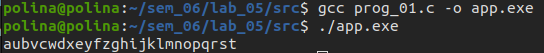
\includegraphics[scale=1.2]{pics/1_1.png}
	\caption{Результат работы первой программы (один поток)}
\end{figure}

\begin{lstlisting}[caption=Программа №1 (два потока)]
#include <fcntl.h>
#include <stdio.h>
#include <unistd.h>
#include <pthread.h>

#define BUF_SIZE 20

void *thread_run(void *fs)
{
	int flag = 1;
	char c;
	while (flag == 1)
	{
		flag = fscanf(fs, "%c", &c);
		if (flag == 1)
		fprintf(stdout, "thread #2: %c\n", c);
	}
	return NULL;
}

int main()
{
	int fd = open("data/alphabet.txt", O_RDONLY);
	pthread_t td;
	
	FILE *fs1 = fdopen(fd, "r");
	char buff1[BUF_SIZE];
	setvbuf(fs1, buff1, _IOFBF, BUF_SIZE);
	
	FILE *fs2 = fdopen(fd, "r");
	char buff2[BUF_SIZE];
	setvbuf(fs2, buff2, _IOFBF, BUF_SIZE);
	
	pthread_create(&td, NULL, thread_run, fs2);
	usleep(1);
	
	int flag = 1;
	char c;
	while (flag == 1)
	{
		flag = fscanf(fs1, "%c", &c);
		if (flag == 1)
		fprintf(stdout, "thread #1: %c\n", c);
	}
	pthread_join(td, NULL);
	
	return 0;
}
\end{lstlisting}

На рисунке 1.2 представлен результат работы первой программы.

\begin{figure}[H]
	\centering
	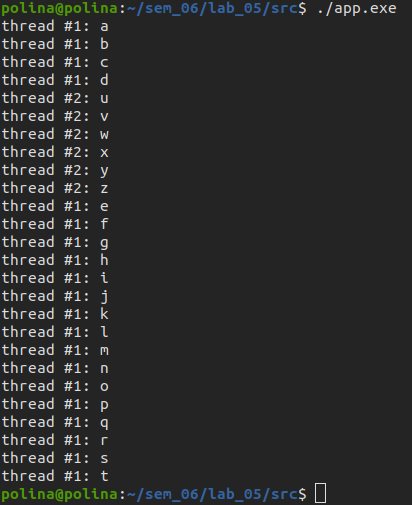
\includegraphics[scale=1]{pics/1_2.png}
	\caption{Результат работы первой программы (два потока)}
\end{figure}

\section{Анализ}

На рисунке 1.3 представлена схема структур, используемых в первой программе.

\begin{figure}[H]
	\centering
	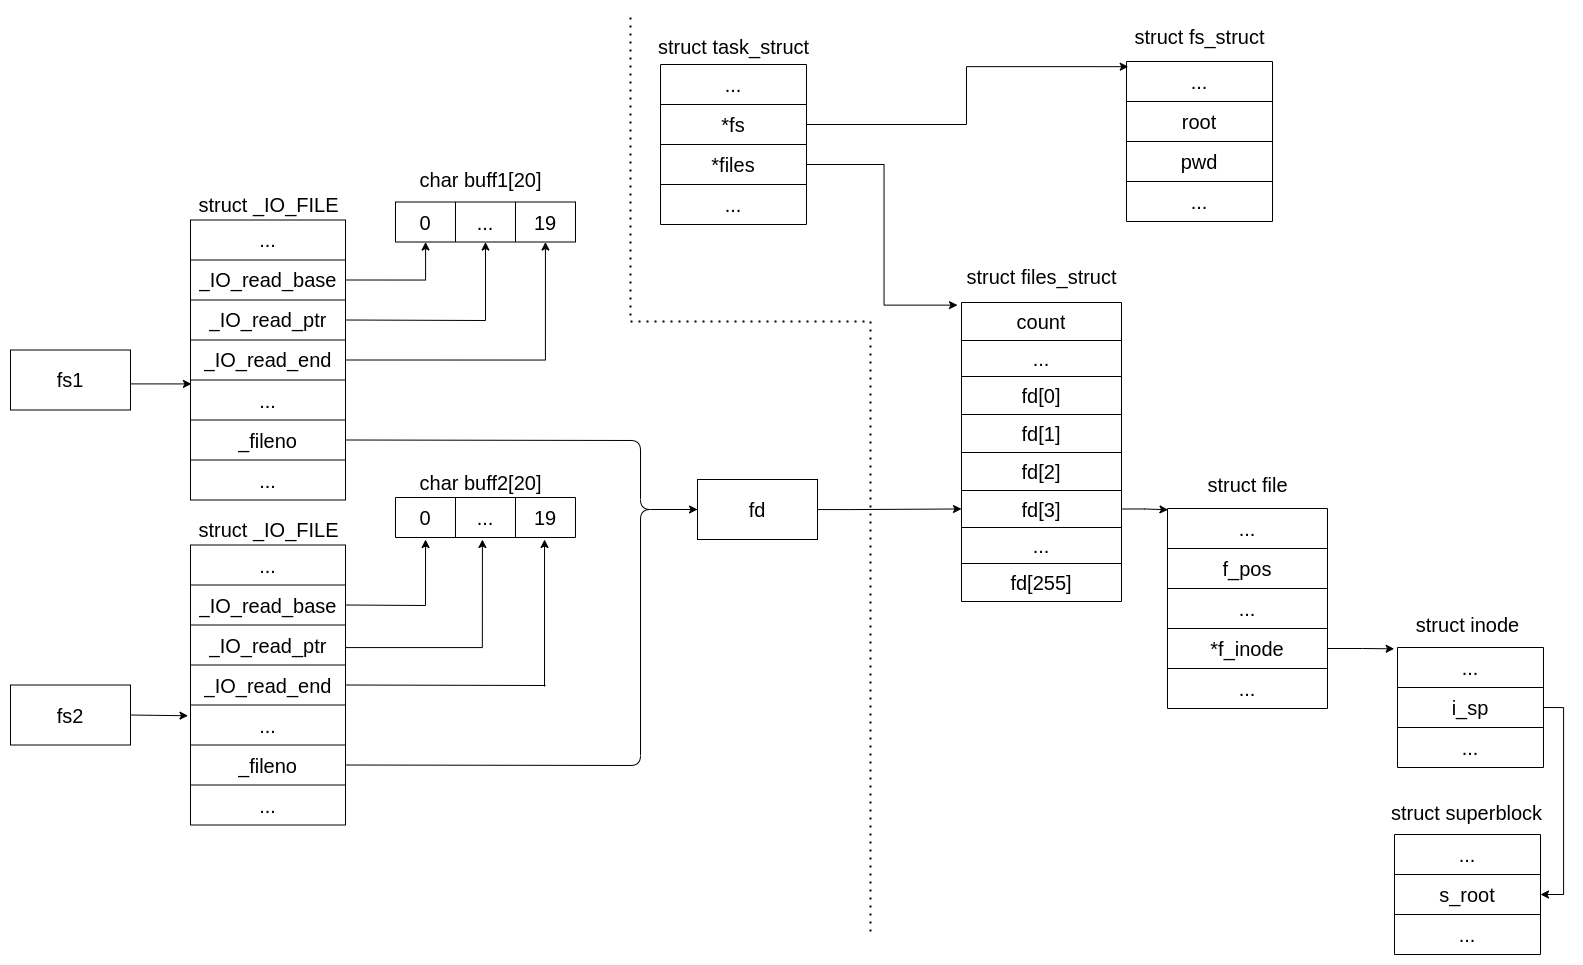
\includegraphics[scale=0.32]{pics/d1.png}
	\caption{Схема структур, используемых в первой программе}
\end{figure}

В начале работы программы системный вызов open() создает и возвращает файловый дескриптор для открытого только на чтение (флаг O\_RDONLY) файла <<data/alphabet.txt>>. Этот системный вызов также создает запись в общесистемной таблице открытых файлов, в которой указаны флаги и смещение в файле. Дескриптор файла является ссылкой на одну из этих записей. Данному файловому дескриптору присваивается значение 3, поскольку значения 0, 1, 2 зарезервированы потоками stdin, stdout, stderr.

В результате вызова fdopen() будут созданы 2 экземпляра структуры FILE (fs1 и fs2), которые ссылаются на дескриптор, созданный ранее в результате системного вызова open(). Создаются буферы buff1 и buff2 размером 20 байт. Для дескрипторов fs1 и fs2 в результате вызова функции setvbuf устанавливаются буферы, а также тип буферизации \_OFBF(полная буферизация).

Затем происходит поочередный вызов функции fscanf() для fs1 и fs2. В виду того, что установлена полная буферизация, при первом вызове fscanf() буфер buff1 заполнится полностью, т.е. будет содержать 20 первых символов алфавита.

В результате вызовов функции fscanf() буфер fs1 заполнится полностью, т.е. первыми 20 символами. Значение f\_pos увеличится на 20.

В результате последующих вызовов функции fscanf() в буфер fs2 считаются оставшиеся 6 символов из алфавита, начиная с f\_pos. 

Затем в результате вызовов функции fprintf() поочередно выводятся символы из buff1 и buff2.

\section{Вторая программа}

\begin{lstlisting}[caption=Программа №2 (один поток)]
#include <fcntl.h>
#include <unistd.h>
#include <stdio.h>

#define OK 0
#define FILE_NAME "data/alphabet.txt"

int main(void)
{
	int fd1 = open(FILE_NAME, O_RDONLY);
	int fd2 = open(FILE_NAME, O_RDONLY);
	int rc1, rc2 = 1;
	
	char c;
	
	while (rc1 == 1 || rc2 == 1)
	{
		if ((rc1 = read(fd1, &c, 1)) == 1)
			write(1, &c, 1);
		
		if ((rc2 = read(fd2, &c, 1)) == 1)
			write(1, &c, 1);
	}
	
	fprintf(stdout, "\n");
	
	return OK;
}
\end{lstlisting}

На рисунке 1.4 представлен результат работы второй программы.

\begin{figure}[H]
	\centering
	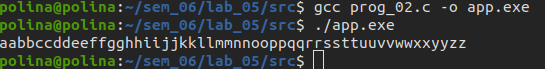
\includegraphics[scale=1.2]{pics/2_1.png}
	\caption{Результат работы второй программы (один поток)}
\end{figure}

\clearpage
\begin{lstlisting}[caption=Программа №2 (два потока)]
#include <fcntl.h>
#include <stdio.h>
#include <unistd.h>
#include <pthread.h>

void *thread_run(void *fs)
{
	int fd = *(int *)fs;
	int rc = 1;
	
	char c;
	while (rc == 1)
	{
		rc = read(fd, &c, 1);
		if (rc == 1)
		write(1, &c, 1);
	}
	
	return NULL;
}

int main()
{
	int fd1 = open("data/alphabet.txt", O_RDONLY);
	int fd2 = open("data/alphabet.txt", O_RDONLY);
	int rc = 1;
	
	pthread_t td;
	pthread_create(&td, NULL, thread_run, &fd2);
	usleep(1);
	
	char c;
	while (rc == 1)
	{
		if ((rc = read(fd1, &c, 1)) == 1) write(1, &c, 1);
	}
	
	pthread_join(td, NULL);
	fprintf(stdout, "\n");
	
	return 0;
}
\end{lstlisting}

На рисунке 1.5 представлен результат работы второй программы (выполнено несколько запусков программы).

\begin{figure}[H]
	\centering
	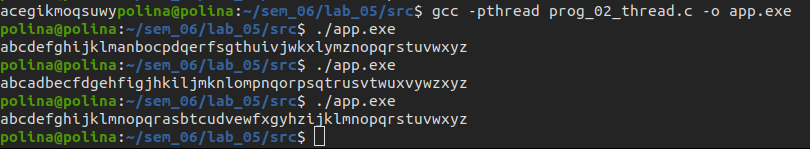
\includegraphics[scale=0.8]{pics/2_2.png}
	\caption{Результат работы второй программы (два потока)}
\end{figure}

\section{Анализ}

На рисунке 1.6 представлена схема структур, используемых во второй программе.

\begin{figure}[H]
	\centering
	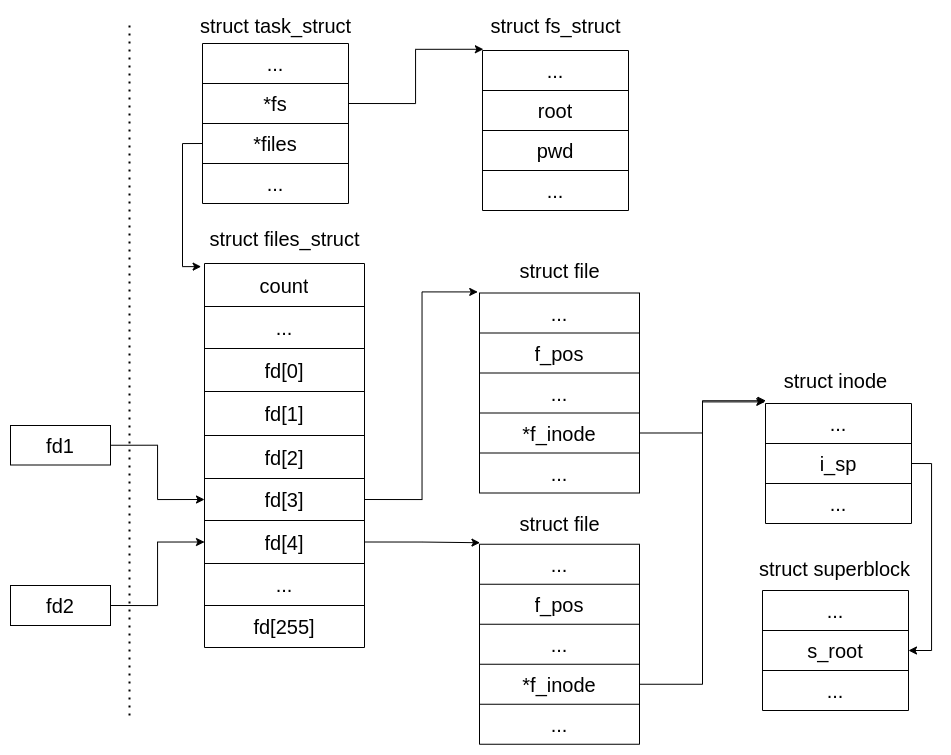
\includegraphics[scale=0.45]{pics/d2.png}
	\caption{Схема структур, используемых во второй программе}
\end{figure}

В начале работы программы в результате двукратного системного вызова open() создается 2 файловых дескриптора для одного и того же текстового файла, открытого только на чтение (O\_RDONLY). Несмотря на то, что файл один и тот же, создаются две разные структуры struct FILE, ссылающиеся на один и тот же struct inode. 

Т.к. созданы два экземпляра структуры, в случае однопоточной реализации посимвольная печать приведет к дублированию каждого символа при выводе на экран. В случае многопоточной реализации символы будут выводиться на экран в перемешанном порядке. Порядок символов вывода не гарантирован, однако алфавит будет выведен целиком.

\section{Третья программа}

\begin{lstlisting}[caption=Программа №3 (один поток)]
#include <fcntl.h>
#include <stdio.h>
#include <unistd.h>

int main()
{
	FILE *fd1 = fopen("data/out.txt", "w");
	FILE *fd2 = fopen("data/out.txt", "w");
	for (char c = 'a'; c <= 'z'; ++c)
	{
		if (c % 2 == 0)
			fprintf(fd1, "%c", c);
		else
			fprintf(fd2, "%c", c);
	}
	fclose(fd1);
	fclose(fd2);
	return 0;
}
\end{lstlisting}

На рисунке 1.7 представлен результат работы третьей программы.

\begin{figure}[H]
	\centering
	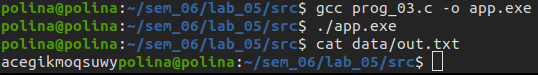
\includegraphics[scale=1.2]{pics/3_1.png}
	\caption{Результат работы третьей программы (один поток)}
\end{figure}

\begin{lstlisting}[caption=Программа №3 (два потока)]
#include <fcntl.h>
#include <stdio.h>
#include <unistd.h>
#include <pthread.h>
#include <sys/stat.h>

void *thread_run(void *fs)
{
	struct stat info;
	
	for (char c = 'a'; c <= 'z'; c += 2)
	{
		fprintf(fs, "%c", c);
	}
	fclose(fs);
	stat("data/out.txt", &info);
	fprintf(stdout, "fclose data/out.txt for fd2: inode is %ld, buffsize is %ld, blocksize is %ld\n", info.st_ino, info.st_size, info.st_blksize);
	
	return NULL;
}

int main()
{
	struct stat info;
	
	FILE *fd1 = fopen("data/out.txt", "w");
	stat("data/out.txt", &info);
	fprintf(stdout, "fopen #1 data/out.txt for fd1: inode is %ld, buffsize is %ld, blocksize is %ld\n", info.st_ino, info.st_size, info.st_blksize);
	
	FILE *fd2 = fopen("data/out.txt", "w");
	stat("data/out.txt", &info);
	fprintf(stdout, "fopen #2 data/out.txt for fd1: inode is %ld, buffsize is %ld, blocksize is %ld\n", info.st_ino, info.st_size, info.st_blksize);
	
	pthread_t td;
	pthread_create(&td, NULL, thread_run, fd2);
	
	for (char c = 'b'; c <= 'z'; c += 2)
	{
		fprintf(fd1, "%c", c);
	}
	fclose(fd1);
	stat("data/out.txt", &info);
	fprintf(stdout, "fclose data/out.txt for fd1: inode is %ld, filesize is %ld, blocksize is %ld\n", info.st_ino, info.st_size, info.st_blksize);
	pthread_join(td, NULL);
	
	return 0;
}
\end{lstlisting}

На рисунке 1.8 представлен результат работы третьей программы.

\begin{figure}[H]
	\centering
	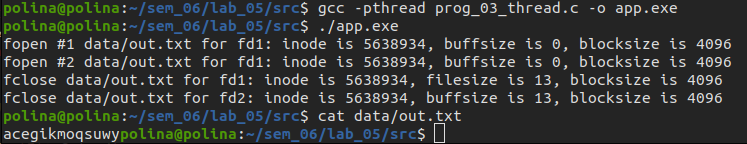
\includegraphics[scale=0.8]{pics/3_2.png}
	\caption{Результат работы третьей программы (два потока)}
\end{figure}

\clearpage
\section{Анализ}

На рисунке 1.9 представлена схема структур, используемых в третьей программе.

\begin{figure}[H]
	\centering
	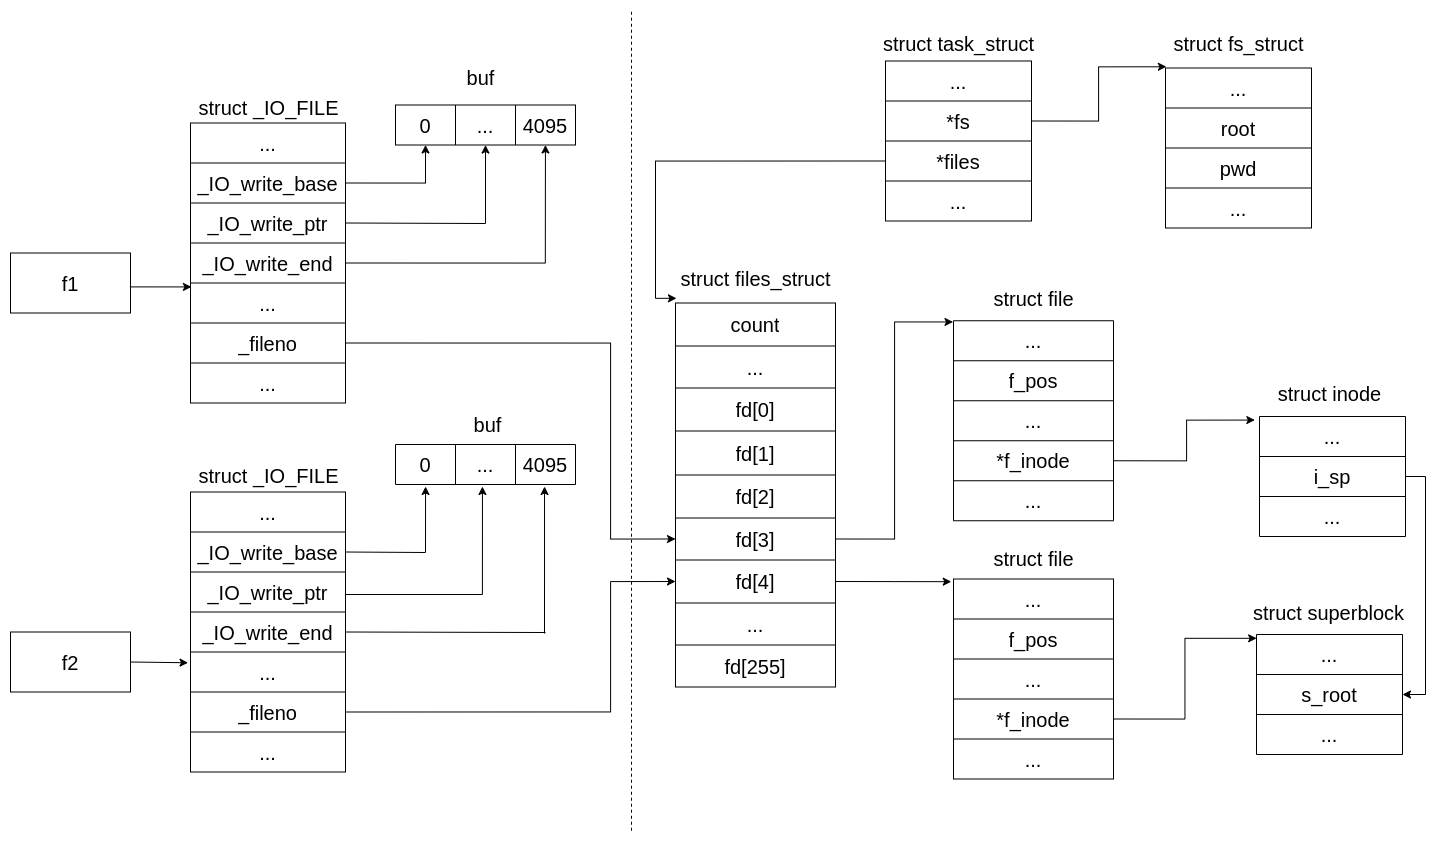
\includegraphics[scale=0.35]{pics/d3.png}
	\caption{Схема структур, используемых в третьей программе}
\end{figure}	

В начале работы программы в результате двукратного вызова библиотечной функции fopen() файл открывается на запись 2 раза. Буфер создается без вмешательства программиста при первой операции записи, его размер равен 4096 байт (размер 1 страницы памяти). По умолчанию используется полная буферизация, при которой запись в файл из буфера произойдет либо при заполнении буфера, либо при вызовe fclose(), либо при завершении процесса.

Вывод выполняется с помощью стандартной функции fprintf()

Информация будет записана в файл в следующих случаях:
\begin{enumerate}
	\item Буфер полон;
	\item Вызвана функция fflush() (Принудительная запись);
	\item Если вызван fclose().
\end{enumerate} 
  
В анализируемой программе информация из буфера запишется в файл в результате вызова fclose().

Т.к. f\_pos независимы у каждого дескриптора файла, то при закрытии файла запись будет производиться начиная с начала файла в обоих случаях. Таким образом информация, которая будет записана в файл, после первого вызова fclose() будет потеряна в результате второго вызова fclose().

%\section*{Выводы}
%
%В ходе выполнения лабораторной работы были проанализированы три программы, демонстрирующие особенности работы функций ввода-вывода в UNIX/Linux.
	
\end{document}